\documentclass[titlepage,a4paper]{article}
\usepackage[nottoc,numbib]{tocbibind}
\usepackage{graphicx}
\usepackage{float}
\usepackage[utf8]{inputenc}


\title{
\Huge{Comparison of algorithms for automated university scheduling}
    \bigskip
	\large{
	\textbf{Supervisor:} Pawel Herman \\
	DD143X Degree project in Computer Science \\
	School of Computer Science and Communication \\
	Kungliga Tekniska Högskolan
	}
}


 
\author{
\textbf{Group 31} \\
Hugo Sandelius, hugosa@kth.se \\ 
Simon Forssell, sifo@kth.se \\
}

\begin{document}
\maketitle

\begin{abstract}
Lorem ipsum dolor sit amet, consectetur adipisicing elit, sed do eiusmod tempor incididunt ut labore et dolore magna aliqua. Ut enim ad minim veniam, quis nostrud exercitation ullamco laboris nisi ut aliquip ex ea commodo consequat. Duis aute irure dolor in reprehenderit in voluptate velit esse cillum dolore eu fugiat nulla pariatur. Excepteur sint occaecat cupidatat non proident, sunt in culpa qui officia deserunt mollit anim id est laborum	
\end{abstract}

\tableofcontents{}

\pagebreak
\section{Introduction}
Timetables are used in many different areas, for example:

\begin{itemize}

  \item Public transport timetables - a list of times and routes connecting places. Travelers can use this to plan how to go from point A to point B.
  \item Broadcast scheduling - used by television and radio stations to schedule when shows and commercials are broadcasted. Often certain shows are to be broadcasted at the same time every day or week.
  \item University timetables - listing all the classes together with time and location so that students know when and where to be. 

\end{itemize}
To put together a good timetable is a complex problem and it is very hard to do by hand. A multitude of factors need to be taken into account, e.g. not having one person do two different tasks at the same time, or to spread out a different tasks across a schedule. It is not surprising that we let computers do this for us. In fact the problem is so complex there probably does not even exist an algorithm that will create an optimal timetable in a reasonable amount of time. This is because this timetabling problem belongs to a class of problems called \emph{NP-hard}\cite{guidedSearch09}  and a consequence of this is that as the problem size grows, the time it takes to find an optimal solution increases exponentially. \\\\
This means that it will not be possible to find an optimal solution, instead an approximate solution must be searched for. But it is not immediately clear what an optimal solution is. What an optimal solution means certainly differs depending on what the timetable is going to be used for. This report will look into what makes a good university timetable and also go over a few methods of how to generate one. \\\\
The report will compare how well two different scheduling algorithms perform for scheduling problems of different sizes. The time taken to generate schedules of various sizes will be assessed, as well as how the solution changes over the running time of the algorithm. This gives an idea of how long time it takes to generate solutions of varying quality. \\\\
First the report will measure how well the algorithm performs on a small problem size, and then see how well it scales up when applied to a significantly larger problem size.
The problems will be artificially generated by us, with inspiration from how the input files to the KTH scheduling department looks, and will be defined in more detail in the Method section. \\\\
The following algorithms will be compared, each of which address the problem from a separate angle.\\\\
\emph{Tabu Search} is a variant of a local search algorithm, which does a local search around at a solution’s neighbours to try and find better solutions. It complements this with marking certain areas as “tabu”, which means it should not be visited again\cite{aTabuSearch07}. \\\\
\emph{Genetic algorithms} mimics the biological process of natural selection. These two are well-known and commonly used algorithms for timetabling\cite{guidedSearch09}. \\\\
Tabu Search and Genetic Algorithms are both algorithms that are commonly used for optimization problems. Since this is a core part of the scheduling problem, they are commonly used for this task. There is also a lot of existing literature about using them for timetable generation. They have two quite different approaches to solving the problem, and thus would be interesting to compare.
These algorithms will be described in detail in the Background section.

\pagebreak
\section{Background}
Automated timetabling is a very well researched subject, especially in the university setting. There are numerous reports written on the various aspects of this topic, most of them in the form of detailed descriptions of algorithms solving the timetabling problem. A few examples are \emph{An Application of Genetic Algorithms to University Timetabling} by A. Brownlee from 2005 and \emph{A Guided Search Genetic Algorithm for the University Course Timetabling Problem} by S. N. Jat and S Yang from 2009. Both are used as source material for this report. \\\\
Although timetabling problems have been studied since the 1960s\cite{efficient03}, the first computer-enabled timetabling systems were established in the late 1980s\cite{timeTableInfo06}. For traffic planning, there are a number of widely-used systems. Currently used systems are for example \emph{HAFAS}, used in the European railway sector, and \emph{EFA}, used for local traffic planning in many European cities. These uses graph-based approaches, using versions of Dijkstra’s Algorithm combined with heuristics to try and find a good approximation of the shortest path between two physical positions\cite{timeTableInfo06}. \\\\
However, for university timetabling, most universities have developed their own solution\cite{efficient10}. The scale of the problem, as well as the constraints involved, vary widely and so does the solution approaches. However, the core of any timetabling algorithm is a combinatorial problem that must be solved by some algorithm. Some of the different algorithms that can be commonly found in timetabling litterature are \emph{local search techniques}, \emph{Tabu search}, \emph{genetic algorithms}, \emph{constraint programming} and \emph{goal programming}\cite{efficient03}. \\\\
Genetic Algorithms and Tabu Search represent two quite different approaches to the problem, although they both utilize an evaluation function to evaluate the solution in each step, and have a current best solution which is improved as the algorithm iterates.

\subsection{Genetic Algorithms}
Genetic algorithms are a part of a larger group of algorithms, Evolutionary algorithms, all inspired by the processes of natural evolution. Artificial evolution was first used in the 1950s by Nils Aall Barricelli in his work \emph{Symbiogenetic evolution processes realized by artificial method}. Most of the research was theoretical until the 1980s when the massive growth of available computational power allowed for practical applications of these methods. \\\\
Genetic algorithms work on a set of potential solutions. This set is called a population and each solution is represented by a chromosome. Every separate property of a specific solution is stored in the string of genes making up the chromosome. The algorithm starts off with an, often randomly generated, initial solution. A function then calculates the fitness of each chromosome by evaluating the chromosome’s solution. Chromosomes with high fitness have a higher chance of being selected for “breeding” and thereby passing on their genes to the next generation of the population. When creating the new population several genetic operators could be used, for example crossover or mutation.  \\\\
\textbf{Crossover} generates new chromosomes by swapping genes between two or more parent chromosomes. There are different ways of selecting which genes to swap. Picking some point in the gene string and swapping all genes beyond that point or swapping all genes within some interval are two common methods. It is also possible to randomly swap genes so that the probability of a swap is set by a mixing rate. \\\\
\textbf{Mutation} works by changing the values of the genes to something other than their initial values. Whether a gene should be changed or not is determined by probability\cite{anApp05}. \\\\
The process then starts over again with calculating the fitness of each chromosome. The average quality of the solutions will probably increase with every new generation. The population continues to evolve like this until an optimal solution is found, the number of iterations reaches a set limit, or some other stopping condition is met. \\\\
\subsection{Tabu Search}
Tabu Search is a search algorithm that was originally formalized by Fred W. Glover in 1989\cite{tabuSearch89}. \\\\
Tabu Search is a local search algorithm. Local searches takes a possible solution to a problem and evaluate its’ neighbors, by assigning an evaluation score to each of them, in order to see if they are a better solution. Neighbors in this case means solutions with some minor difference from the solution in question. If a neighbor has a higher evaluation score, and thus is a better solution, it becomes the new current solution, and in the next iteration neighbors to this solution is evaluated. This continues until some stopping criteria is fulfilled, similar to genetic algorithms. \\\\
Picking which neighbors should be evaluated in each iteration is a key part of local search algorithms, and this is where Tabu Search comes in.
In Tabu Search, we keep track of previously visited solutions in a tabu list. Any solution in the tabu list will not be visited again until a certain condition has been fulfilled, for example a certain number of solutions having been visited. This keeps the local search from getting stuck in a local optimum or a plateau, and helps it expand the search to other regions\cite{geneticVS99}. 

\pagebreak
\section{Method}
A program is developed that takes user input, consisting of course information and constraints, and generates schedules using two different algorithms as they are described in the Background section. The input consists of a list of classrooms and their capacities, a list of programs and their courses, and the lessons in each course, with each lesson being assigned a teacher and a number of students in the lesson. The total amount of weeks the schedule should be planned for is also included.
The schedules assigns lessons to four possible slots each day. \\\\
The hard constraints, i. e. the ones which has to be fulfilled by the algorithm, if possible, are:
\begin{itemize}
  \item All lessons must be assigned a time
  \item A classroom must hold at least as many students as are planned for the lesson
  \item Only one lesson in one program at the same time
  \item A teacher may only teach one class at a time
\end{itemize} 
\medskip
The soft constraints, which are used to evaluate the schedule but are not absolute, are:
\begin{itemize}
  \item The amount of free periods, i.e. unscheduled time between classes in a day, should be minimized
  \item There should preferably not be more than one lesson in the same course in a day
\end{itemize}
\medskip
AAfter the schedule is generated, the program will assess how well the various soft constraints were fulfilled. If a perfect schedule, i. e. one where all soft and hard constraints are fulfilled, can be generated in a reasonable time, the amount of time and iterations of each algorithm will be compared. \\\\
Two different input files of increasing sizes will be used to generate the schedules. The input files are artificial, but constructed with inspiration from how the input to the KTH scheduling system works.
How well the different algorithms scale with increasingly complex input will then be studied.
The small input file features 3 programmes with between 2 and 4 courses. Each course has between 7 and 15 lessons.
The large input file features 6 programmes, each with between 3 and 5 courses. Each course has between 15 and 20 lessons.
Since both algorithms has elements of randomness they are run 10 times with each input file, after which the average result is calculated, to avoid the impact of chance on the algorithms. \\\\
The Tabu Search algorithm will be implemented as described in the theory section. The neighbors are generated in two ways, by changing the classroom of a random lesson to a random new classroom, and by swapping the time of two lessons. The possible swaps and changes will be calculated at random. The solutions in the tabu list is then excluded from the neighbors. When researching how well the algorithms scale, the tabu list will have a size of 10 solutions, and each solution will remain in the tabu list until 10 more solutions have been evaluated. \\\\
The chromosomes of the genetic algorithm are set up using genes with integer values. Each gene corresponds to a classroom and a point in time. The value of the gene represents the activity scheduled there. The initial chromosomes are completely randomized. The only genetic operator used in the algorithm is a mutation operator that randomly swaps the values of the genes within the chromosome. The population size used for the scaling tests will be 60. \\\\
Tabu Search and Genetic Algorithms both use an evaluation function to evaluate the different solutions as they are searching for the best one. To ensure a fair comparison of the algorithms, the same evaluation function will be used for both algorithms. \\\\
The way Tabu Search and the Genetic Algorithm approaches a perfect solution will aslo be researched by looking at how the evaluation score changes with each iteration. \\\\
The Tabu Search and Genetic Algorithms algorithms have several different parameters that affect how the algorithm works. Evaluation of how varying these parameters influence the results of the algorithms will also be done to figure out if the comparison of the algorithms holds in general, or just for a specific implementation of them.
For Tabu Search, the parameters are the tabu list size and the amount of neighbors evaluated in each iteration. 
In the genetic algorithm, the only parameter is the size of the population.

\pagebreak
\section{Results}
\subsection{Scaling}
For the small input file, both algorithms could create a perfect schedule (i. e. one which fulfills all hard and soft constraints) in a reasonable time. In an average of 10 runs, tabu search needed 461 iterations in 10.465 seconds, while the genetic algorithm needed on average 974 iterations in 13.183 seconds. \\\\
For the large-sized input file, the tabu search could create a perfect schedule in 862 iterations, or 72.285 seconds. When run for 5000 iterations ten times, the genetic algorithm only managed to create a perfect schedule four times, the average for these four runs was 2774 iterations or 414.584 seconds. In all other cases the algorithm was one single broken constraint away from a perfect schedule. \\\\

\begin{figure}[H]
  \centering
    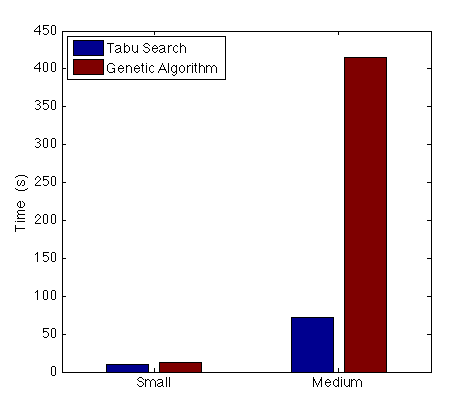
\includegraphics[scale=0.5]{../results/time_bar_graph.png}
  \caption{Running time for the small and large sized problems with both algorithms.}
  \label{time_bar_graph}
\end{figure}

\subsection{Evaluation score development}
The evaluation score varies during one running of the algorithm as follows: \\\\
\begin{figure}[H]
  \centerline{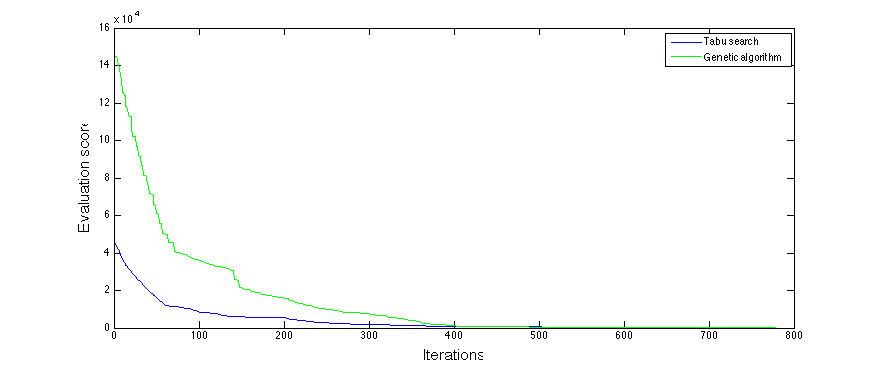
\includegraphics[scale=0.5]{../results/plot_small.png}}
  \caption{Small file.}
  \label{plot_small}
\end{figure}

\begin{figure}[H]
  \centerline{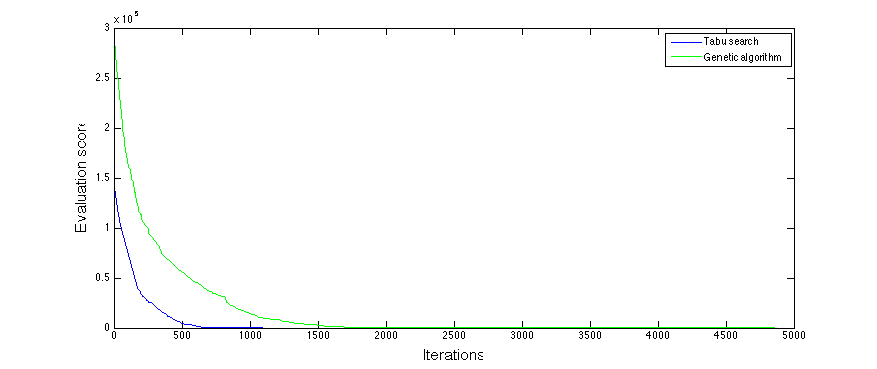
\includegraphics[scale=0.5]{../results/plot_medium.png}}
  \caption{Large file.}
  \label{plot_large}
\end{figure}

\begin{figure}[H]
  \begin{center}
    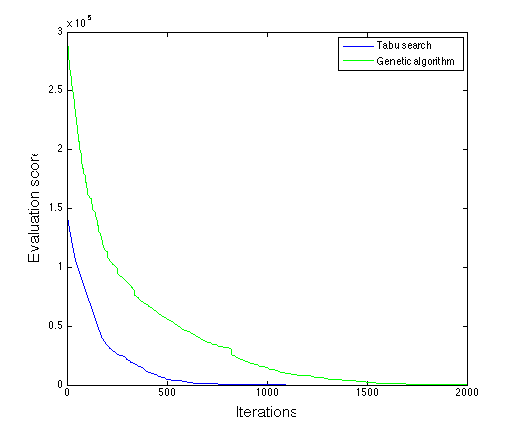
\includegraphics[scale=0.6]{../results/plot_medium_zoomed.png}
  \end{center}
  \caption{A closer look at the first 2000 iterations of the runs with the large file.}
  \label{plot_large_zoomed}
\end{figure}

\subsection{Algorithm parameters}
These graphs portray how the running time was influenced by varying the various parameters to the algorithms. Particularly, it shows how long time it took, on an average over 10 runs, to solve the small constraints file when the parameters are varied. \\\\
\begin{figure}[H]
  \begin{center}
    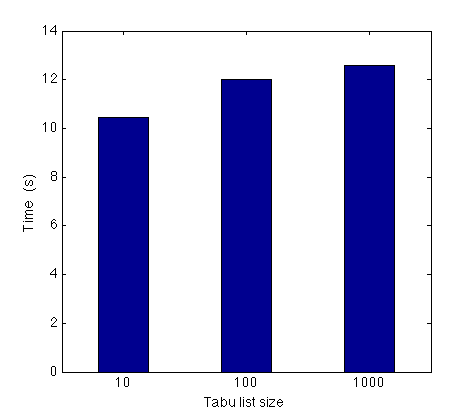
\includegraphics[scale=0.5]{../results/tabu_list_size.png}
  \end{center}
  \caption{The running time of the tabu search for the small file varying the tabu list size.}
  \label{tabu_list_size}
\end{figure}

\begin{figure}[H]
  \begin{center}
    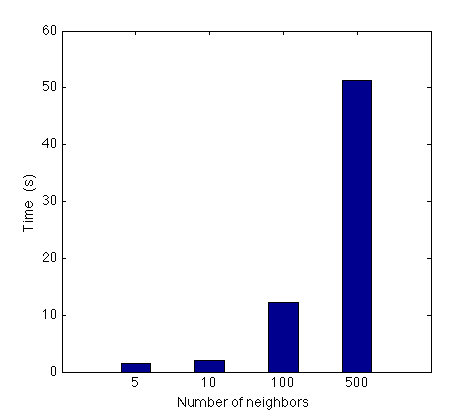
\includegraphics[scale=0.5]{../results/tabu_neighbor.png}
  \end{center}
  \caption{The running time of the tabu search for the small file varying the number of neigbors.}
  \label{tabu_neighbor}
\end{figure}

\begin{figure}[H]
  \begin{center}
    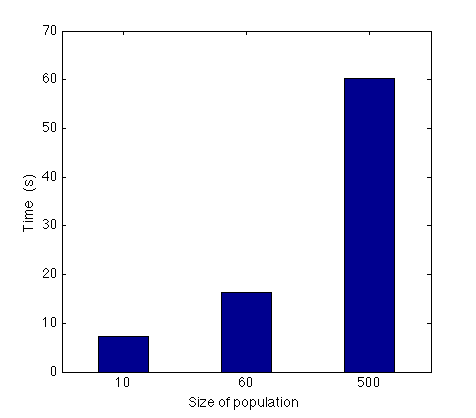
\includegraphics[scale=0.5]{../results/genetic_population.png}
  \end{center}
  \caption{The running time of the genetic algorithm for the small file varying the size of the population.}
  \label{genetic_pop}
\end{figure}

\pagebreak
\section{Discussion}
In the small input size, the algorithms are fairly close in running time, with Tabu Search having a slight edge. However, as the input size is increased to large, the Genetic Algorithms are much slower. Looking at the evaluation score development makes it clearer what is happening. The Genetic Algorithms have a worse solution at all times during the run, but when there are only very few broken constraints left, the algorithm is having a lot of trouble satisfying these constraints. This means that it will usually take a long time to find a perfect solution, and sometimes it can get stuck on solving the final few constraints for a very long time.
Also of note is that the Tabu Search has a notable “corner”, after a certain points the constraints start to get solved at a slower rate, while the Genetic Algorithm slows down over a longer time, and tends to make significant progress in certain “jumps”. \\\\
The amount of neighbors generated and visited each iteration in Tabu Search makes the running time vary greatly. When fewer neighbors are evaluated at a time, the Tabu Search runs for more iterations and changes the current optimal solution more often, while less time is spent finding a good neighbor to iterate to. This seems to be more efficient for the input data used in this project.
The Tabu List size, on the contrary, has relatively little impact on the running time. It is possible having a longer Tabu List is simply not worth it due to the larger overhead of dealing with the larger list. \\\\
Varying the population size of the genetic algorithms has a major impact on the time it takes to find an optimal solution. When increasing the size of the population the number of potential solutions managed by the algorithm grows and with that the diversity of the solutions. This could potentially lead to finding better solutions in fewer iterations. However, it appears that the increased time it takes for the algorithm to handle all these solutions outweigh the advantage of a greater diversity among the solutions. \\\\
It should be noted that the implementation of the algorithms certainly has an impact on their running time, as can be seen with the wild variations of running time when some of the algorithm parameters are changed. However, effort has been made to stay close to standard implementations of the algorithms as described in literature.

\pagebreak
\section{Conclusion}
For typical university scheduling problems, with the implementations of the algorithms used in this report, Tabu Search scales better to larger scheduling problems, while Genetic Algorithms is slower and will, for larger problems, have problems satisfying the last few constraints. The amount of neighbors visited in each iteration during Tabu Search should be low for an optimal algorithm, and the population size in the genetic algorithm should also be kept relatively small.

\pagebreak

\bibliographystyle{plain}
\bibliography{sources}
\end{document}